\documentclass{article}
\paperwidth 35cm

\usepackage{xeCJK}
\usepackage{tikz}
\usetikzlibrary{arrows.meta} % 自定义箭头样式
\usetikzlibrary{shapes.misc} % 图形库
\usetikzlibrary{shapes.geometric} % 图形库
\usetikzlibrary{shadings} % 渐变色
\usetikzlibrary{shadows} % 阴影
\usetikzlibrary{positioning} % 提供node的位置描述特性
\usepackage{xcolor}

%%% the color is amazing!!! %%%

\pagestyle{empty}
\begin{document}

\tikzstyle{sysBase} = [
  shape=rectangle, rounded corners=3mm,
  shade, ball color=green, drop shadow,
  text badly centered, inner sep=4mm]
\tikzstyle{sys1} = [
  sysBase, top color=blue, bottom color=blue, middle color=white
]
\tikzstyle{sys2} = [
  sysBase, top color=white, bottom color=blue,
]

\section{my design}
\tikz{
  \node[sys1] (st1)  at (0,0) {\Huge{存储管理分系统}};
  \node[sys2, right=of st1] {\Huge{任务管理分系统}};   
  \node[sys1, below=of st1,left color=green, right color=green, middle color=white!80]  {应用处理子系统};  

}

\section{xcolor}
\definecolor{myc1}{rgb}{0.2,0.4,0.8}
\colorlet{myc12}{blue!10} % let myc12= rgb:0.5,0.1,0
\definecolorset{rgb}{x-}{-y}{red,1,0,0;green,0,1,0;blue,0,0,1}

\begin{testcolors}[rgb,cmyk,hsb,HTML,gray]
\testcolor{myc1}
\testcolor{myc12}
\testcolor{x-red-y}
\testcolor{x-green-y}
\testcolor{x-blue-y}
\testcolor{red!10!green!10!blue}
\testcolor{red!20!green!20!blue}
\testcolor{red!30!green!30!blue}
\testcolor{red!40!green!40!blue}
\testcolor{red!50!green!50!blue}
\testcolor{red!60!green!60!blue}
\testcolor{red!70!green!70!blue}
\testcolor{red!80!green!80!blue}
\testcolor{red!90!green!90!blue}
\testcolor{red}
\testcolor{red!75}
\testcolor{red!75!green}
\testcolor{red!75!green!50}
\testcolor{red!75!green!50!blue}
\testcolor{red!75!green!50!blue!25}
\testcolor{red!75!green!50!blue!25!gray}

\testcolor{rgb:red,4; green,4; blue,1}
\testcolor[hsb]{0.4,0.8,0.4}
\testcolor[cmyk]{0,0,.5,.5}
%\testcolor[rgb:cmyk]{0,0,.5,.5}
\end{testcolors}


\section{node}
\tikz{
  \node[draw,
    shape=isosceles triangle, % shape: circle, triangle
    fill=red,text=yellow
  ] at (0,0) {\Huge{ node style test}};

  \node[shade, top color=yellow,  bottom color=green, middle color=red % middle color must after top and bottom color
    ,shape=rectangle, rounded corners=1mm
    , scale=2] at (0,-4) {shade 1};

  \node[shade, left color=yellow, right color=green, middle color=red
    ,shape=rectangle, rounded corners=2mm
    , scale=2] at (4, -4) {shade 2};

  \node[shade, ball color=green
    ,shape=rectangle, rounded corners=3mm
    , scale=2] at (8, -4) {shade 3};

  \node[
    %% shade, ball color=green,
    shape=rectangle, rounded corners=3mm,
    draw, drop shadow={opacity=0.3},
    scale=2] at (0, -6) {shadow 1};

  \node[
    %shade, ball color=green,
    shape=rectangle, rounded corners=3mm,
    copy shadow, fill=green!20, draw=blue,
    scale=2] at (4, -6) {shadow 2};

  \node[draw=black,
    shape=circle, rounded corners=5mm,
    circular drop shadow,
    scale=2] at (8, -6) {shadow 3};
}\\
\tikz{
    % node tree;
  \node {node name}
  child {node {child node}}
  child {node {child node2}}
  ;
}


\section{Arrows}
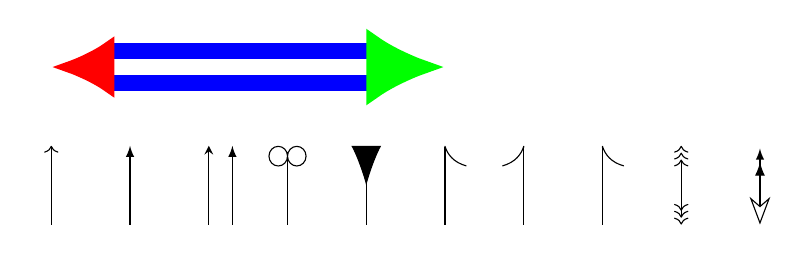
\begin{tikzpicture} [xxx /.tip={Latex[sep] latex[sep]},
    yyy /.tip={Stealth[length=10pt, open]}
  ]
  \draw [->] (0,0) -- (0, 1);
  \draw [-{stealth}] (2,0) -- (2,1);
  \draw [-{latex}] (1,0) -- (1,1);
  \draw [-latex] (2.3,0) -- (2.3, 1);
  \draw [arrows={-Hooks[arc=360, scale=3]}] (3,0) -- (3, 1); % 向左右然后向后弯曲的箭头,终点弯曲的角度为360度,360度就弯成圆圈了
  \draw [arrows={-Latex[reversed, scale=3]}] (4,0) -- (4,1); % 反向箭头
  \draw [arrows={->[harpoon, swap, scale=3]}] (5,0) -- (5,1); % harpoon箭头, swap研箭头方向为轴镜像
  \draw [arrows={->[left, scale=3]}] (6,0) -- (6,1); % 左半边
  \draw [arrows={->[right, scale=3]}] (7,0) -- (7,1); % 右半边
  \draw [<.<<->.>>] (8,0) -- (8,1);
  \draw [{yyy}-{xxx}] (9,0) -- (9,1);
  \draw [line width=2mm, double distance=2mm, color=blue,
    arrows={{Latex[width=8mm,length=8mm, color=red]}-{Latex[width=5mm,length=5mm, scale=2, color=green]}}
  ] (0,2) -- (5,2);
% [«.<-.»>] 
  
\end{tikzpicture}


\section{连线测试}
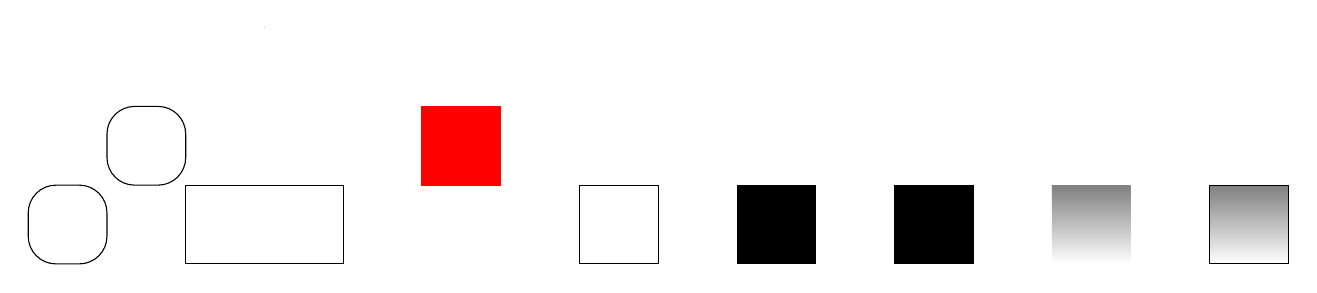
\begin{tikzpicture}
  \path [draw, rounded corners=10pt] (0,0) rectangle (1,1) (1,1) rectangle (2,2); % 多个path可以放在一行中写

  \path (4,1) rectangle (2,0) [draw]; % [] 参数的位置可以在开头,中间和结尾,建议结尾
  \path [draw] (5,1) rectangle (6,2) [fill, red] ; %参数可以分开写

  \draw (7,0) rectangle (8,1) ; % draw 表示画框线, fill表示填充
  \fill (9,0) rectangle (10,1);
  \filldraw (11,0) rectangle (12,1);
  \shade (13,0) rectangle (14,1); % shade 渐变?
  \shadedraw (15,0) rectangle (16,1);
  \clip (2,2) rectangle (3,3); % ?
  \useasboundingbox (4,2) rectangle (5,3);
  
  \draw [color=red, very thin] (3,3) rectangle (4,4);
  \node {root}
  child {node {no1}}
  child {node {no2}
    child {node {nxx1}}
    child {node {nxx2}}
  };
  
      
\end{tikzpicture}


\end{document}
